\documentclass[]{article}
\usepackage{lmodern}
\usepackage{amssymb,amsmath}
\usepackage{ifxetex,ifluatex}
\usepackage{fixltx2e} % provides \textsubscript
\ifnum 0\ifxetex 1\fi\ifluatex 1\fi=0 % if pdftex
  \usepackage[T1]{fontenc}
  \usepackage[utf8]{inputenc}
\else % if luatex or xelatex
  \ifxetex
    \usepackage{mathspec}
  \else
    \usepackage{fontspec}
  \fi
  \defaultfontfeatures{Ligatures=TeX,Scale=MatchLowercase}
\fi
% use upquote if available, for straight quotes in verbatim environments
\IfFileExists{upquote.sty}{\usepackage{upquote}}{}
% use microtype if available
\IfFileExists{microtype.sty}{%
\usepackage{microtype}
\UseMicrotypeSet[protrusion]{basicmath} % disable protrusion for tt fonts
}{}
\usepackage{hyperref}
\hypersetup{unicode=true,
            pdftitle={Emacs em 30 Segundos},
            pdfauthor={Guaracy Monteiro},
            pdfborder={0 0 0},
            breaklinks=true}
\urlstyle{same}  % don't use monospace font for urls
\usepackage{color}
\usepackage{fancyvrb}
\newcommand{\VerbBar}{|}
\newcommand{\VERB}{\Verb[commandchars=\\\{\}]}
\DefineVerbatimEnvironment{Highlighting}{Verbatim}{commandchars=\\\{\}}
% Add ',fontsize=\small' for more characters per line
\newenvironment{Shaded}{}{}
\newcommand{\KeywordTok}[1]{\textcolor[rgb]{0.00,0.44,0.13}{\textbf{{#1}}}}
\newcommand{\DataTypeTok}[1]{\textcolor[rgb]{0.56,0.13,0.00}{{#1}}}
\newcommand{\DecValTok}[1]{\textcolor[rgb]{0.25,0.63,0.44}{{#1}}}
\newcommand{\BaseNTok}[1]{\textcolor[rgb]{0.25,0.63,0.44}{{#1}}}
\newcommand{\FloatTok}[1]{\textcolor[rgb]{0.25,0.63,0.44}{{#1}}}
\newcommand{\ConstantTok}[1]{\textcolor[rgb]{0.53,0.00,0.00}{{#1}}}
\newcommand{\CharTok}[1]{\textcolor[rgb]{0.25,0.44,0.63}{{#1}}}
\newcommand{\SpecialCharTok}[1]{\textcolor[rgb]{0.25,0.44,0.63}{{#1}}}
\newcommand{\StringTok}[1]{\textcolor[rgb]{0.25,0.44,0.63}{{#1}}}
\newcommand{\VerbatimStringTok}[1]{\textcolor[rgb]{0.25,0.44,0.63}{{#1}}}
\newcommand{\SpecialStringTok}[1]{\textcolor[rgb]{0.73,0.40,0.53}{{#1}}}
\newcommand{\ImportTok}[1]{{#1}}
\newcommand{\CommentTok}[1]{\textcolor[rgb]{0.38,0.63,0.69}{\textit{{#1}}}}
\newcommand{\DocumentationTok}[1]{\textcolor[rgb]{0.73,0.13,0.13}{\textit{{#1}}}}
\newcommand{\AnnotationTok}[1]{\textcolor[rgb]{0.38,0.63,0.69}{\textbf{\textit{{#1}}}}}
\newcommand{\CommentVarTok}[1]{\textcolor[rgb]{0.38,0.63,0.69}{\textbf{\textit{{#1}}}}}
\newcommand{\OtherTok}[1]{\textcolor[rgb]{0.00,0.44,0.13}{{#1}}}
\newcommand{\FunctionTok}[1]{\textcolor[rgb]{0.02,0.16,0.49}{{#1}}}
\newcommand{\VariableTok}[1]{\textcolor[rgb]{0.10,0.09,0.49}{{#1}}}
\newcommand{\ControlFlowTok}[1]{\textcolor[rgb]{0.00,0.44,0.13}{\textbf{{#1}}}}
\newcommand{\OperatorTok}[1]{\textcolor[rgb]{0.40,0.40,0.40}{{#1}}}
\newcommand{\BuiltInTok}[1]{{#1}}
\newcommand{\ExtensionTok}[1]{{#1}}
\newcommand{\PreprocessorTok}[1]{\textcolor[rgb]{0.74,0.48,0.00}{{#1}}}
\newcommand{\AttributeTok}[1]{\textcolor[rgb]{0.49,0.56,0.16}{{#1}}}
\newcommand{\RegionMarkerTok}[1]{{#1}}
\newcommand{\InformationTok}[1]{\textcolor[rgb]{0.38,0.63,0.69}{\textbf{\textit{{#1}}}}}
\newcommand{\WarningTok}[1]{\textcolor[rgb]{0.38,0.63,0.69}{\textbf{\textit{{#1}}}}}
\newcommand{\AlertTok}[1]{\textcolor[rgb]{1.00,0.00,0.00}{\textbf{{#1}}}}
\newcommand{\ErrorTok}[1]{\textcolor[rgb]{1.00,0.00,0.00}{\textbf{{#1}}}}
\newcommand{\NormalTok}[1]{{#1}}
\usepackage{graphicx,grffile}
\makeatletter
\def\maxwidth{\ifdim\Gin@nat@width>\linewidth\linewidth\else\Gin@nat@width\fi}
\def\maxheight{\ifdim\Gin@nat@height>\textheight\textheight\else\Gin@nat@height\fi}
\makeatother
% Scale images if necessary, so that they will not overflow the page
% margins by default, and it is still possible to overwrite the defaults
% using explicit options in \includegraphics[width, height, ...]{}
\setkeys{Gin}{width=\maxwidth,height=\maxheight,keepaspectratio}
\IfFileExists{parskip.sty}{%
\usepackage{parskip}
}{% else
\setlength{\parindent}{0pt}
\setlength{\parskip}{6pt plus 2pt minus 1pt}
}
\setlength{\emergencystretch}{3em}  % prevent overfull lines
\providecommand{\tightlist}{%
  \setlength{\itemsep}{0pt}\setlength{\parskip}{0pt}}
\setcounter{secnumdepth}{0}
% Redefines (sub)paragraphs to behave more like sections
\ifx\paragraph\undefined\else
\let\oldparagraph\paragraph
\renewcommand{\paragraph}[1]{\oldparagraph{#1}\mbox{}}
\fi
\ifx\subparagraph\undefined\else
\let\oldsubparagraph\subparagraph
\renewcommand{\subparagraph}[1]{\oldsubparagraph{#1}\mbox{}}
\fi

\title{Emacs em 30 Segundos}
\author{Guaracy Monteiro}
\date{}

\begin{document}
\maketitle

{
\setcounter{tocdepth}{3}
\tableofcontents
}
\pagebreak

\begin{center}\rule{0.5\linewidth}{\linethickness}\end{center}

\textbf{TL;DR}

Arquivo de configuração para ser utilizado em uma instalação nova do
Emacs ou substituir uma antiga (excluir \textbf{.emacs} e
\textbf{.emacs.d}). Automaticamente instala alguns pacotes definidos e
configura o ambiente e os pacotes. Tudo bem explicadinho para ser
alterado//melhorado facilmente.

\begin{enumerate}
\tightlist
\item
  Grave o arquivo
  \href{https://raw.githubusercontent.com/guaracy/emacs/master/config/.emacs}{.emacs},
  no seu diretório \textbf{home}. Se desejar, grave também o arquivo
  \href{https://raw.githubusercontent.com/guaracy/emacs/master/config/.myemacs}{.myemacs}
  no seu diretório \textbf{home}. Abra o Emacs e espere a configuração
  terminar.
\item
  Baixe e leia a documentação \textbf{TBD} .
\end{enumerate}

\begin{center}\rule{0.5\linewidth}{\linethickness}\end{center}

\pagebreak

\section{Emacs em 30 segundos}\label{emacs-em-30-segundos}

A ideia base deste projeto é a possível dificuldade de instalação e
configuração do Emacs por parte dos usuários. A instalação é simples
mas, conforme o programa sai de \emph{fábrica}, muitas pessoas encontram
uma pequena dificuldade inicial e, como pensam: ``- \emph{Ah, é só mais
um editor de textos. Vou continuar com o que eu já conheço}.'', e perdem
uma ferramenta das mais poderosas que poderiam usar. Apesar de ser
possível efetuar algumas alterações pelo menu, muitas necessitam que o
usuário edite um arquivo de configuração (\textbf{.emacs}). A instalação
de novos pacotes, por exemplo, já foi uma tarefa bem mais complicada.

\subsection{Alternativas}\label{alternativas}

Existem algumas opções que possuem um Emacs configurado para o usuário
final. É possível citar:

\begin{enumerate}
\tightlist
\item
  \href{https://github.com/syl20bnr/spacemacs}{Spacemacs} : É uma ótima
  alternativa e bastante indicada para usuários do Vim. Existem pessoas
  que tentaram usar o Emacs mas voltaram para o Vim. Depois de instalar
  o Spacemacs, estão usando é achando ótimo. Basicamente é uma cópia do
  diretório \textbf{.emacs.d} com toda a configuração automática. O
  usuário precisará ler a documentação se desejar fazer alguma alteração
  na configuração.
\item
  \href{https://github.com/myTerminal/super-emacs}{super-emacs} : Também
  é uma cópia do diretório \textbf{.emacs.d} porém com uma configuração
  mais simples que o Spacemacs.
\item
  \href{https://github.com/ergoemacs/ergoemacs-mode}{Ergoemacs} : Deve
  ser uma ótima configuração para o Windows. No Linux é difícil de
  testar pois muitos atalhos conflitam com o desktop (KDE, Gnome, etc).
\item
  \href{https://github.com/guaracy/emacs/tree/master/config}{Emacs30} :
  Este que você está lendo. Baseia-se apenas em uma arquivo de
  configuração (\textbf{.emacs}) que deve ser gravado no diretório home
  do usuário. Ele irá baixar e configurar os diversos pacotes. Ao
  término, ele verifica se existe o arquivo (\textbf{.myemacs}). Se
  existir, continua a configuração por este arquivo.
\end{enumerate}

Vejo como principal desvantagem dos itens 1 e 2 a não habilitação do
CUA-mode. Esconder o menu principal também pode ser estranho para alguns
usuários iniciantes. O item e eu não testei. A habilitação do CUA-mode,
entre outras coisas, permite combinações que a maioria dos usuários está
acostumada como: \emph{Ctrl+c} \emph{Ctrl+c} para copiar, \emph{Ctrl+c}
\emph{Ctrl+v} para colar e \emph{Ctrl+z} para desfazer.

Inicialmente o Emacs possui uma tela assim:

\begin{figure}[htbp]
\centering
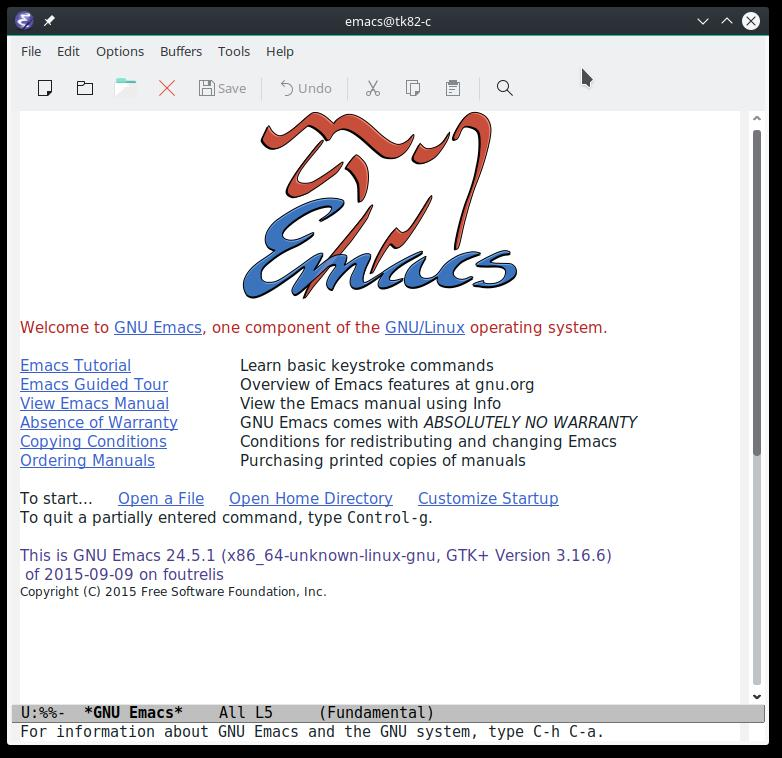
\includegraphics{./images/emacs1.jpg}
\caption{Tela inicial do Emacs}
\end{figure}

ou seja, uma barra de ferramentas de gosto duvidoso (depois de um breve
período de uso você vai achar melhor os atalhos do que tirar a mão do
teclado, pegar o mouse e clicar em um botão) e uma tela inicial com
muita informação. Mas tudo isto irá mudar.

\subsection{Características do
projeto}\label{caracteruxedsticas-do-projeto}

\begin{enumerate}
\tightlist
\item
  Habilitação do CUA-mode para que o usuário não precise aprender que
  \emph{Alt+w} é usada para copiar um texto, por exemplo.
\item
  Alterar a aparência do Emacs, utilizando um tema com fundo escuro. O
  usuário poderá optar por um fundo claro a qualquer momento
\item
  Deixar a barra de status com uma aparência mais agradável.
\item
  Alterar diversas opções para deixar o Emacs mais amigável(?).
\item
  Instalar alguns pacotes para facilitar o trabalho do usuário em
  diversas áreas, podendo inclusive gerar arquivos .docx (Microsoft
  Word), .odt (LibreOffice), .pdf, .epub (eBook) entre diversos outros
  de forma simples (pode necessitar da instalação de programas externos
  como por exemplo, para gerar .pdf é necessário instalar o
  \textbf{MiKTeX} no Windows ou o \textbf{texlive} no Linux).
\end{enumerate}

\subsection{org-mode}\label{org-mode}

Inicialmente estava previsto a instalação do pacote \textbf{markdown}
para facilitar a criação e transformação de textos em uma linguagem de
marcação simples para outros documentos mais complexos. Como o Emacs já
vem com o org-mode e muitos usuários utilizam o Emacs basicamente pelo
pacote, nada melhor do que utilizá-lo.

\begin{enumerate}
\tightlist
\item
  Utiliza uma linguagem de marcação relativamente simples.
\item
  É possível utilizar como arquivo de entrada e exportar para diversos
  formatos.
\item
  De brinde, o usuário ganha um poderoso organizador pessoal que permite
  até a sincronização dos dados com seu smartphone ou tablet.
\item
  Por último mas não menos importante, o GitHub aceita diretamente um
  arquivo README.org como o README.md.
\end{enumerate}

\section{Arquivo .emacs}\label{arquivo-.emacs}

\subsection{Configurações iniciais}\label{configurauxe7uxf5es-iniciais}

\subsection{Pacotes}\label{pacotes}

É onde tudo acontece. Achei que seria melhor explicar com mais detalhes
tudo o que acontece durante a execução do arquivo para que o usuário
possa efetuar alterações básicas para deixar o Emacs mais ao seu gosto.
As linhas que iniciam com ponto e vírgula indicam que são comentários e
não serão interpretadas. Para um entendimento melhor, seria interessante
que o usuário aprendesse um pouco sobre a linguagem \textbf{emacs-lisp}
(uma variação de lisp) de onde vem toda a flexibilidade do Emacs.

\subsubsection{Alterações das opções
iniciais}\label{alterauxe7uxf5es-das-opuxe7uxf5es-iniciais}

Deixei estas alterações no início pois, se for feita alguma alteração
utilizando o menu \textbf{Options} e o usuário selecionar
\textbf{Options/Save Options}, esta parte do arquivo \textbf{.emacs}
será alterada. Ficando no início é mais fácil de visualizar e não causa
tanta confusão.

\begin{Shaded}
\begin{Highlighting}[]
\NormalTok{(custom-set-variables}
 \NormalTok{'(cua-mode }\KeywordTok{t} \KeywordTok{nil} \NormalTok{(cua-base)) (ref:cua)}
 \NormalTok{'(custom-enabled-themes (}\KeywordTok{quote} \NormalTok{(misterioso))) (ref:theme)}
 \NormalTok{'(indicate-empty-lines }\KeywordTok{t}\NormalTok{) (ref:empty)}
 \NormalTok{'(show-paren-mode }\KeywordTok{t}\NormalTok{) (ref:paren)}
 \NormalTok{'(tool-bar-mode }\KeywordTok{nil}\NormalTok{)) (ref:tool)}
\end{Highlighting}
\end{Shaded}

Ativamos o CUA-mode \emph{(cua)}, inicializamos um tema (cores
utilizadas para fundo, fontes e salientar diversas sintaxes no texto)
diferente do original \emph{(theme)}, indicamos que linha vazias devem
conter um símbolo no início para diferencia de linhas que possuam espaço
\emph{(empty)}, dizemos que queremos uma visualização para abertura e
fechamento de chaves, parêntesis e colchetes (muito útil para
programação)\emph{(paren)} e, finalmente, que não desejamos ver a barra
de ferramentas (as teclas de atalho são mais eficientes e nada que dois
níveis do menu não resolvam) \emph{(tool)}.

\subsubsection{Inclusão e atualização de fonte de
pacotes}\label{inclusuxe3o-e-atualizauxe7uxe3o-de-fonte-de-pacotes}

\begin{Shaded}
\begin{Highlighting}[]
\NormalTok{(}\KeywordTok{require} \NormalTok{'package)}
\NormalTok{(add-to-list 'package-archives}
             \NormalTok{'(}\StringTok{"melpa"} \NormalTok{. }\StringTok{"http://melpa.milkbox.net/packages/"}\NormalTok{)}
             \KeywordTok{t}\NormalTok{)}
\NormalTok{(package-initialize)}
\end{Highlighting}
\end{Shaded}

Adiciona o repositório MELPA que contém um maior número de pacotes e com
uma atualização constante.

\begin{Shaded}
\begin{Highlighting}[]
\NormalTok{(}\KeywordTok{when} \NormalTok{(}\KeywordTok{not} \NormalTok{package-archive-contents)}
  \NormalTok{(package-refresh-contents))}
\end{Highlighting}
\end{Shaded}

Atualiza o conteúdo das fontes de pacotes se não existe. Para você
atualizar os pacotes, utilize o menu \textbf{Options/Manage Emacs
Packages}. Na janela de gerenciamento de pacotes, pressione \textbf{U}
para atualizar os pacotes (irá excluir o anterior e instalar a versão
nova), \textbf{I} para instalar algum pacotes desejado (veja
\textbf{.myemacs}), \textbf{D} para excluir algum pacote (atenção para o
que você excluir) e, quando tudo estiver pronto, pressione \textbf{X}
para executar as ações de inclusão e exclusão.

\subsubsection{Seleção e instalação dos pacotes pelo
Emacs30}\label{seleuxe7uxe3o-e-instalauxe7uxe3o-dos-pacotes-pelo-emacs30}

\begin{Shaded}
\begin{Highlighting}[]
\NormalTok{(}\KeywordTok{defvar}\FunctionTok{ gbm-required-packages}
  \NormalTok{'(which-key}
    \NormalTok{hl-line+}
    \NormalTok{powerline}
    \NormalTok{hlinum}
    \NormalTok{hiwin}
    \NormalTok{ido-grid-mode}
    \NormalTok{ido-select-window}
    \NormalTok{imenu-anywhere}
    \NormalTok{smex}
    \NormalTok{pandoc-mode}
    \NormalTok{org-cua-dwim}
    \NormalTok{org-pandoc}
    \NormalTok{auto-complete}
    \NormalTok{smartparens}
    \NormalTok{goto-chg}
    \NormalTok{indent-guide}
    \NormalTok{theme-looper))}
\end{Highlighting}
\end{Shaded}

Não inclua nenhum pacote neste ponto. Utilize o arquivo
\textbf{.myemacs} se deseja incluir outros pacotes. Para saber mais
sobre cada pacote especificado, você pode ir no
\href{https://melpa.org/}{MELPA}, digitar o nome do pacote e clicar no
link da coluna \emph{source}. Na grande maioria das vezes, você irá para
uma página com informações do pacote. No gerenciador de pacotes do
Emacs, \textbf{Options/Manage Emacs Packages}, também existem
informações sobre a finalidade.

\begin{Shaded}
\begin{Highlighting}[]
\NormalTok{(}\KeywordTok{mapc} \NormalTok{(}\KeywordTok{lambda} \NormalTok{(p)}
        \NormalTok{(package-install p))}
      \NormalTok{gbm-required-packages)}
\end{Highlighting}
\end{Shaded}

\subsection{Configurações da aparência e dos
pacotes}\label{configurauxe7uxf5es-da-aparuxeancia-e-dos-pacotes}

\subsubsection{Tamanho da janela}\label{tamanho-da-janela}

\begin{Shaded}
\begin{Highlighting}[]
\NormalTok{(}\KeywordTok{setq} \NormalTok{initial-frame-alist}
      \NormalTok{'(}
        \NormalTok{(width . }\DecValTok{130}\NormalTok{) }\CommentTok{; characters}
        \NormalTok{(height . }\DecValTok{40}\NormalTok{) }\CommentTok{; lines}
        \NormalTok{))}
\end{Highlighting}
\end{Shaded}

Especifica uma altura/largura maior do que os valores padrões. Em muitos
casos, é melhor maximizar a janela para poder trabalhar com mais de um
frame e uma boa visibilidade de cada um.

\subsubsection{Which key}\label{which-key}

\begin{Shaded}
\begin{Highlighting}[]
\NormalTok{(which-key-mode)}
\NormalTok{(which-key-setup-minibuffer)}
\NormalTok{(}\KeywordTok{setq} \NormalTok{max-mini-window-height }\DecValTok{10}\NormalTok{)}
\NormalTok{(}\KeywordTok{setq} \NormalTok{which-key-idle-delay }\FloatTok{0.5}\NormalTok{)}
\NormalTok{(set-face-attribute 'which-key-local-map-description-face }\KeywordTok{nil} \NormalTok{:weight 'bold)}
\end{Highlighting}
\end{Shaded}

Quando o usuário utilizar um atalho como \emph{Ctrl+c} ou \emph{Ctrl+h},
por exemplo, e não digitar o complemento dentro de 0.5 segundos, o
minibuffer irá mostrar as possibilidades existentes para completar o
comando. Foi configurado que o minibuffer terá 10 linhas de altura, o
tempo de espera é de 0,5 segundos e as combinações válidas para o buffer
onde o usuário está trabalhando estarão em negrito.

\subsubsection{Numeração das linhas}\label{numerauxe7uxe3o-das-linhas}

\begin{Shaded}
\begin{Highlighting}[]
\NormalTok{(global-linum-mode }\KeywordTok{t}\NormalTok{)}
\end{Highlighting}
\end{Shaded}

Indica para numerar as linhas em todos os buffers. A qualquer momento o
usuário poderá alterar pressionando \emph{Alt+x linum-mode}.

\subsubsection{Realça linha do cursor}\label{realuxe7a-linha-do-cursor}

\begin{Shaded}
\begin{Highlighting}[]
\NormalTok{(hl-line-mode }\KeywordTok{t}\NormalTok{)}
\NormalTok{(toggle-hl-line-when-idle)}
\NormalTok{(set-face-attribute hl-line-face }\KeywordTok{nil} \NormalTok{:background }\StringTok{"Grey25"}\NormalTok{)}
\NormalTok{(set-cursor-color }\StringTok{"yellow"}\NormalTok{)}
\end{Highlighting}
\end{Shaded}

Irá realçar a linha onde encontra-se o cursor apenas quando o usuário
não estiver fazendo nada. Escolhi \emph{Grey25} como cor de fundo e
\emph{yellow} para a cor do cursor. Para ver as cores, suas combinações
bem como o nome, basta entrar com \emph{Alt+x list-colors-display}

\subsubsection{Realça numeração da linha do
cursor}\label{realuxe7a-numerauxe7uxe3o-da-linha-do-cursor}

\begin{Shaded}
\begin{Highlighting}[]
\NormalTok{(}\KeywordTok{require} \NormalTok{'hlinum)}
\NormalTok{(hlinum-activate)}
\end{Highlighting}
\end{Shaded}

O realce de linha não realça a numeração da linha. A função do
\emph{hlinum} é para realçar o número da linha. Sempre será realçada,
independente do programa estar em espera.

\subsubsection{Realçar parêntesis}\label{realuxe7ar-paruxeantesis}

\begin{Shaded}
\begin{Highlighting}[]
\NormalTok{(show-paren-mode)}
\end{Highlighting}
\end{Shaded}

Realça os respectivos pares de parêntesis, chaves ou colchetes.

\subsubsection{Esconde barra de rolamento
\#\#}\label{esconde-barra-de-rolamento}

\begin{Shaded}
\begin{Highlighting}[]
\NormalTok{(scroll-bar-mode -}\DecValTok{1}\NormalTok{)}
\end{Highlighting}
\end{Shaded}

Esconde a barra de rolamento do frame. A barra de status já possui
informações sobre inicio ou final de arquivo ou percentual que já foi
rolado. Também possui um pequeno ícone mostrando a posição relativa
(como uma mini barra de rolamento). Ganhamos mais um pouco de espaço na
horizontal e menos um elemento para distrair.

\subsubsection{Salva estado atual ao
sair}\label{salva-estado-atual-ao-sair}

\begin{Shaded}
\begin{Highlighting}[]
\NormalTok{(}\KeywordTok{require} \NormalTok{'saveplace)}
\NormalTok{(setq-default save-place }\KeywordTok{t}\NormalTok{)}
\NormalTok{(}\KeywordTok{setq} \NormalTok{save-place-file (expand-file-name }\StringTok{".places"} \NormalTok{user-emacs-directory))}
\end{Highlighting}
\end{Shaded}

Salva a posição atual do cursor no arquivo. Na próxima vez que for
aberto, será posicionado na posição que estava antes de encerra.

\subsubsection{Desabilita buffer de mensagem
inicial}\label{desabilita-buffer-de-mensagem-inicial}

\begin{Shaded}
\begin{Highlighting}[]
\NormalTok{(}\KeywordTok{setq} \NormalTok{initial-buffer-choice}
    \KeywordTok{t}\NormalTok{)}
\end{Highlighting}
\end{Shaded}

Desabilita a tela de abertura que contém diversas informações
desnecessárias.

\subsubsection{Troca mensagem do buffer de
rascunho}\label{troca-mensagem-do-buffer-de-rascunho}

\begin{Shaded}
\begin{Highlighting}[]
\NormalTok{(}\KeywordTok{setq} \NormalTok{initial-scratch-message}
    \StringTok{";; Nada neste buffer será salvo. Use:}\NormalTok{\textbackslash{}n}\StringTok{;;}
\StringTok{    Ctrl+x Ctrl+r / Ctrl+x Ctrl+f para ler um arquivo.}\NormalTok{\textbackslash{}n}\StringTok{"}\NormalTok{)}
\end{Highlighting}
\end{Shaded}

Alterei a mensagem do buffer de rascunho. Nada do que for escrito nele
será salvo automaticamente ao sair. Buffers contendo arquivos, se forem
alterados e ainda não foram salvos ao encerrar o programa, será mostrada
uma mensagem informando que os dados não foram salvos e se o usuário
deseja sair, salvar ou cancelar.

\subsubsection{Realça frame ativo}\label{realuxe7a-frame-ativo}

\begin{Shaded}
\begin{Highlighting}[]
\NormalTok{(}\KeywordTok{require} \NormalTok{'hiwin)}
\NormalTok{(hiwin-activate)}
\NormalTok{(set-face-background 'hiwin-face }\StringTok{"black"}\NormalTok{)}
\end{Highlighting}
\end{Shaded}

Todos os frames visíveis ficarão com o fundo preto, menos o que estiver
ativo.

\subsubsection{Configura powerline}\label{configura-powerline}

\begin{Shaded}
\begin{Highlighting}[]
\NormalTok{(powerline-center-theme)}
\NormalTok{(}\KeywordTok{setq} \NormalTok{powerline-default-separator}
      \NormalTok{'wave)}
\end{Highlighting}
\end{Shaded}

Confere uma apresentação melhor para a linha de status.

\subsubsection{ido no modo grade}\label{ido-no-modo-grade}

\begin{Shaded}
\begin{Highlighting}[]
\NormalTok{(}\KeywordTok{setq} \NormalTok{ido-enable-flex-matching }\KeywordTok{t}\NormalTok{)}
\NormalTok{(}\KeywordTok{setq} \NormalTok{ido-everywhere }\KeywordTok{t}\NormalTok{)}
\NormalTok{(ido-mode }\KeywordTok{t}\NormalTok{)}
\NormalTok{(ido-grid-mode }\KeywordTok{t}\NormalTok{)}
\NormalTok{(global-set-key (kbd }\StringTok{"C-x o"}\NormalTok{) 'ido-select-window)}
\NormalTok{(global-set-key (kbd }\StringTok{"<f4>"}\NormalTok{) 'ido-select-window)}
\end{Highlighting}
\end{Shaded}

IDO (InteractivelyDoThings) mostra as opções disponíveis no minibuffer
facilitando a escolha pelo usuário. Se for informado o comando para
abrir um arquivo (\emph{Ctrl+x Ctrl+f}) por exemplo, será aberto um
frame com a relação dos arquivos e diretórios para que seja feita a
escolha. A última escolha sempre aparecerá em primeiro lugar. O usuário
poderá usar as setas e enter para selecionar o arquivo ou poderá ir
digitando o nome do arquivo ficando visíveis apenas os que coincidirem
com o digitado. Se o diretório tiver diversos arquivos com o nome
\emph{temp} e extensões diferentes (supondo-se que nenhum inicie com o
caractere \emph{t}), basta digitar \emph{t} e parte da extensão:
\emph{ttex} selecionará todos os arquivos que possuam a extensão
iniciando com /tex'.

\subsubsection{\texorpdfstring{Configura atalho \textbf{Ctrl+.} para
imenu-anywhere}{Configura atalho Ctrl+. para imenu-anywhere}}\label{configura-atalho-ctrl.-para-imenu-anywhere}

\begin{Shaded}
\begin{Highlighting}[]
\NormalTok{(global-set-key (kbd }\StringTok{"C-."}\NormalTok{) 'imenu-anywhere)}
\end{Highlighting}
\end{Shaded}

Mostra no minibuffer, via IDO, o que o programa acha que é interessante
para que o usuário possa movimentar-se com mais rapidez no arquivo. Nome
de funções e procedimentos no caso de programas, o que for considerado
título em arquivos texto, etc.

\subsubsection{\texorpdfstring{Configura atalhos \textbf{Alt+x} e
\textbf{Alt+X} para
smex}{Configura atalhos Alt+x e Alt+X para smex}}\label{configura-atalhos-altx-e-altx-para-smex}

\begin{Shaded}
\begin{Highlighting}[]
\NormalTok{(global-set-key (kbd }\StringTok{"M-x"}\NormalTok{) 'smex)}
\NormalTok{(global-set-key (kbd }\StringTok{"M-X"}\NormalTok{) 'smex-major-mode-commands)}
\end{Highlighting}
\end{Shaded}

Se o usuário digitar \emph{Alt+x}, será apresentado no minibuffer via
IDO, uma seleção das possíveis complementações.

\subsubsection{Configura o autocomplete}\label{configura-o-autocomplete}

\begin{Shaded}
\begin{Highlighting}[]
\NormalTok{(ac-config-default)}
\NormalTok{(ac-linum-workaround)}
\end{Highlighting}
\end{Shaded}

Apresenta um menu para completar automaticamente a digitação de funções
e procedimentos em programas. Quando existente, apresenta uma janela de
auxílio sobre a função//procedimento atual.

\subsubsection{Indent guide}\label{indent-guide}

\begin{Shaded}
\begin{Highlighting}[]
\NormalTok{(indent-guide-global-mode)}
\end{Highlighting}
\end{Shaded}

Mostra barras verticais para mostras a endentação em programas.

\subsubsection{Configura theme-looper}\label{configura-theme-looper}

\begin{Shaded}
\begin{Highlighting}[]
\NormalTok{(theme-looper-set-theme-set '(adwaita}
                              \NormalTok{deeper-blue}
                              \NormalTok{dichromacy}
                              \NormalTok{misterioso}
                              \NormalTok{tango-dark}
                  \NormalTok{tango}
                  \NormalTok{tsdh-dark}
                              \NormalTok{wheatgrass}
                              \NormalTok{wombat))}

\NormalTok{(theme-looper-set-customizations 'powerline-reset)}
\NormalTok{(global-set-key (kbd }\StringTok{"C-}\NormalTok{\textbackslash{}"}\StringTok{"}\NormalTok{) 'theme-looper-enable-next-theme)}
\end{Highlighting}
\end{Shaded}

Permite que o usuário passeie pelos temas especificado para verificar
algum que lhe agrade mais. Para alterar definitivamente, uma das opções
é ir no menu \textbf{Options/Customize Emacs/Custom Themes}.

\subsubsection{Configura goto last
change}\label{configura-goto-last-change}

\begin{Shaded}
\begin{Highlighting}[]
\NormalTok{(global-set-key (kbd }\StringTok{"C-x ."}\NormalTok{) 'goto-last-change)}
\NormalTok{(global-set-key (kbd }\StringTok{"C-x ,"}\NormalTok{) 'goto-last-change-reverse)}
\end{Highlighting}
\end{Shaded}

Permite que o usuário pule nas últimas alterações Pressionando a
combinmação /Ctrl+,/ e \emph{Ctrl+.}.

\subsubsection{Ctrl+x Ctrl+r abre lista de arquivos
recentes}\label{ctrlx-ctrlr-abre-lista-de-arquivos-recentes}

\begin{Shaded}
\begin{Highlighting}[]
\NormalTok{(}\KeywordTok{require} \NormalTok{'recentf)}
\NormalTok{(recentf-mode }\KeywordTok{t}\NormalTok{)}
\NormalTok{(}\KeywordTok{setq} \NormalTok{recentf-max-menu-items }\DecValTok{25}\NormalTok{)}
\NormalTok{(}\KeywordTok{defun}\FunctionTok{ recentf-ido-find-file }\NormalTok{()}
  \StringTok{"Find a recent file using Ido."}
  \NormalTok{(interactive)}
  \NormalTok{(}\KeywordTok{let} \NormalTok{((file (ido-completing-read }\StringTok{"Choose recent file: "} \NormalTok{recentf-list }\KeywordTok{nil} \KeywordTok{t}\NormalTok{)))}
    \NormalTok{(}\KeywordTok{when} \NormalTok{file}
      \NormalTok{(find-file file))))}
\NormalTok{(global-set-key (kbd }\StringTok{"C-x C-r"}\NormalTok{) 'recentf-ido-find-file)}
\end{Highlighting}
\end{Shaded}

Utilizando \emph{Ctrl+x Ctrl+r} permite que o usuário abra um minibuffer
para escolher entre os últimos arquivo editados.

\subsubsection{Carrega arquivo .myemacs}\label{carrega-arquivo-.myemacs}

\begin{Shaded}
\begin{Highlighting}[]
\NormalTok{(}\KeywordTok{setq} \NormalTok{myconfig }\StringTok{"~/.myemacs"}\NormalTok{)}
\NormalTok{(}\KeywordTok{if} \NormalTok{(file-exists-p myconfig)}
    \NormalTok{(load-file myconfig))}
\end{Highlighting}
\end{Shaded}

Informa para ler o conteúdo do arquivo \textbf{.myemacs} se ele existir.
Deverá conter outras configurações desejadas pelo usuário. Não
colocá-las no arquivo \textbf{.emacs}.

\subsubsection{Define F3 para pesquisar e Shift+F3 para pesquisar
próxima}\label{define-f3-para-pesquisar-e-shiftf3-para-pesquisar-pruxf3xima}

\begin{Shaded}
\begin{Highlighting}[]
\CommentTok{;;-----------------------------------------}
\CommentTok{;; Define F3 para iniciar busca}
\CommentTok{;; F3 novamente para próxima ocorrência}
\CommentTok{;; Shift+F3 para ocorrência anterior}
\NormalTok{(global-set-key (kbd }\StringTok{"C-f"}\NormalTok{) 'isearch-forward)}
\NormalTok{(define-key isearch-mode-map (kbd }\StringTok{"<f3>"}\NormalTok{) 'isearch-repeat-forward)}
\NormalTok{(define-key isearch-mode-map (kbd }\StringTok{"S-<f3>"}\NormalTok{) 'isearch-repeat-backward)}
\end{Highlighting}
\end{Shaded}

Permite que o usuário digite \emph{Ctrl+f} para efetuar uma pesquisa ou
invés de \emph{Ctrl+s} que é o padrão do Emacs. Pressionando \emph{F3}
vai para a próxima ocorrência e \emph{Shift+F3} para a ocorrência
anterior.

\subsubsection{TODO Alterar}\label{todo-alterar}

\begin{Shaded}
\begin{Highlighting}[]
\CommentTok{;;------------------------------------------}
\CommentTok{;; ## Movimentação entre frames}
\CommentTok{;;}
\NormalTok{(windmove-default-keybindings) }\CommentTok{;; 'meta);}
\CommentTok{;; Make windmove work in org-mode:}
\NormalTok{(add-hook 'org-shiftup-final-hook 'windmove-up)}
\NormalTok{(add-hook 'org-shiftleft-final-hook 'windmove-left)}
\NormalTok{(add-hook 'org-shiftdown-final-hook 'windmove-down)}
\NormalTok{(add-hook 'org-shiftright-final-hook 'windmove-right)}

\NormalTok{(}\KeywordTok{setq} \NormalTok{org-CUA-compatible }\KeywordTok{t}\NormalTok{)}
\NormalTok{(}\KeywordTok{setq} \NormalTok{org-support-shift-select }\KeywordTok{t}\NormalTok{)}
\NormalTok{(}\KeywordTok{setq} \NormalTok{org-src-fontify-natively }\KeywordTok{t}\NormalTok{)}
\NormalTok{(}\KeywordTok{setq} \NormalTok{org-startup-truncated }\KeywordTok{nil}\NormalTok{)}
\end{Highlighting}
\end{Shaded}

\section{Arquivo .myemacs}\label{arquivo-.myemacs}

\subsubsection{TODO Fazer}\label{todo-fazer}

\end{document}
